\subsubsection{Estensione B: Prezzo Inferiore all’Offerta Originale}

Nel caso in cui l’agente inserisca un prezzo di controproposta inferiore a quello dell’offerta ricevuta, il sistema intercetta l’anomalia e informa immediatamente l’utente dell’errore.

\subsubsection{Validazione del Prezzo e Feedback all’Utente}
Dopo aver cliccato su \textbf{“Invia controproposta”}, viene mostrato un messaggio di errore sotto al campo di input, specificando che il prezzo inserito non può essere inferiore a quello proposto dall’acquirente.  
Il sistema non consente il salvataggio della controproposta fino alla correzione del valore inserito.

Questo comportamento applica il principio della \textbf{prevenzione degli errori}, garantendo coerenza logica nelle transazioni e riducendo la possibilità di offerte incoerenti o non valide.

\begin{figure}[H]
	\centering
	\begin{tikzpicture}[node distance=1.5cm and 1cm, auto]
		% Nodo per immagine 2 con didascalia sotto, posizionato a destra di img1
		\node (img1) {
			\begin{tabular}{c}
				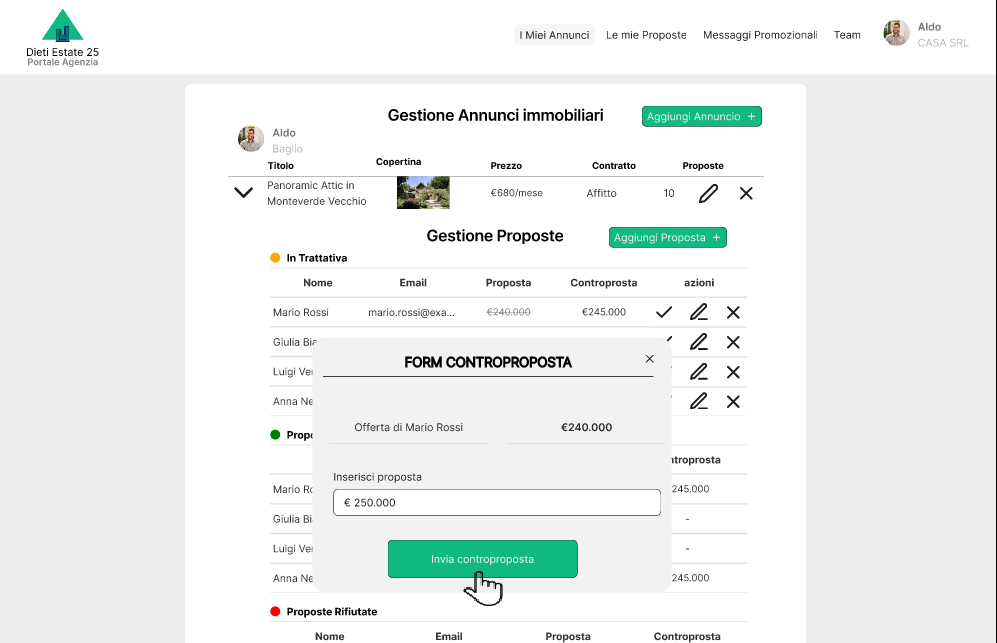
\includegraphics[width=0.7\textwidth]{Immagini/Mockup/controproposte/scenario principale/ClickInviaControproposta.png} \\
				Cockburn: step 7.B
			\end{tabular}
		};
		
		% Nodo per immagine 3 con didascalia sotto, posizionato sotto img2
		\node (img2) [below=of img1] {
			\begin{tabular}{c}
				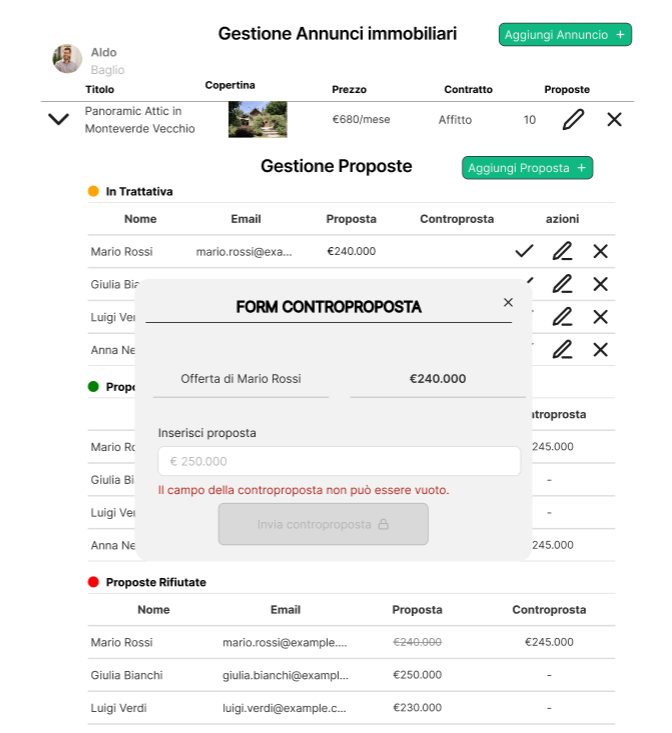
\includegraphics[width=0.7\textwidth]{Immagini/Mockup/controproposte/Extensions B/MessaggioDiErrore.png} \\
				Cockburn: step 8.B
			\end{tabular}
		};
		
		% Disegna le frecce
		\draw[->, thick] (img1) -- (img2);
		
	\end{tikzpicture}
	\caption{Mockup: Extension B della tabella di Cockburn del caso d'uso: Fare una controproposta a un'offerta.}
	\label{fig:tikz_flow}
\end{figure}

\newpage


